\chapter{Background and Theory}
This chapter explores the two general areas of Computer Science that are considered when developing and deploying an Internet of Things platform supporting resource constrained devices. Firstly, we describe the general area of Immersive Participation and its constituent theories around pervasive computing. Secondly we look at the deployment of pervasive middleware in the distributed computing paradigm more closely examining the MediaSense platform as a concrete realisation of this approach. Additionally, we discuss the general trend of pervasive and ubiquitous computing towards resource constraint devices. Finally, we look at the inter procedure communication and more specifically remote method invocation as the theory for extending the MediaSense platform in order to solve the problem shown in section \ref{problem}. 

\section{Immersive Participation}
Immersive participation is focused on participation on the Internet via ubiquitous computing and context-awareness. It enables people, places and things to connect to each other to create Immersive Participation Environments. Immersive Participation Environments provides users with context-awareness everywhere which makes the users participate as if they are in a virtual world with places, things and people in it. Common examples of Immersive Participation Environments today include Google Ingress \cite{ingress} where users join teams and compete with other teams in a virtual world where they need to take over real world artefacts, TURF \cite{turf} where users capture real world places and gain points and RATS Theatre's \cite{rats} application called Maryam \cite{maryam} which is an interactive theater where audio clips is triggered depending on the user's Global Positioning System (GPS) location.

Larger scale immersive applications will benefit from scalable distributed information sharing and also remove bottlenecks and dependencies on centralized web portals on the internet.
The way humans interact with each other and things around them will change when sensor information can be shared and accessed ubiquitously. Creating immersive environments that blend the natural world with a seamless internet of things require that we are able to understand the situation of the users in real-time this understanding is termed context awareness.

\section{Context Awareness}
Improving the computers ability to access and understand a user's circumstances give developers more information for creating  applications that respond and adapt to the user. A way to accomplish this is to not only use data given by the user, but also use context information from the user's environment. According to Dey in \cite{dey2001understanding}, the definition of context is:

\begin{quotation}
\centering
Context is a combination of any information that can be sensed or received by an entity which is useful to catch events and situations.
\end{quotation}

In other words, context is information from an entity that gives specific information to increase the understanding of an events environment. An entity can be a person, place or an object that is relevant for the interaction. 

One way of generating and sharing this context information on a large scale is through the use of smart telephones and other ubiquitous computing devices. One such smartphone is the a Google Nexus 4 \cite{GoogleNexus} which contains, among other things, an accelerometer to detect acceleration, a GPS to receive location data, a gyroscope to detect rotation, a barometer to detect air pressure and a compass for direction and navigation. By applying sensor fusion \cite{Elmenreich02sensorfusion} other context data can be attained. The phone will collect context-information from its GPS sensor and based on this location be able to give directions. With this extra context information, we can create applications that are context aware. This idea of context awareness is summarized by Dey in \cite{dey2001understanding} as: 

\begin{quotation}
\centering
A system is context-aware if it uses context to provide relevant information and \slash or services to the user, where relevancy depends on the user's task.
\end{quotation}

An example of context-awareness in applications is Google Latitude \cite{GoogleLatitude}, where it's possible to see your friends' location on a map, as shown in figure \ref{googlelat}. Other good examples include applications on smartphones and tablets which rotate the image on screen based on the device's physical orientation as shown in figure \ref{androidorientation}.

\begin{figure}[t] % To force on specific place use H
	\centering
    	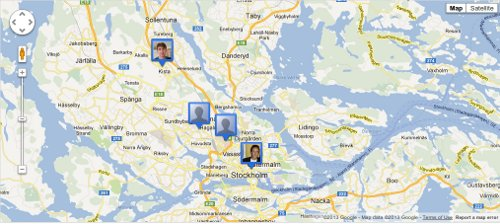
\includegraphics[scale=0.75]{part_2/context_awareness/latitude_pic.jpg}
		\caption{A picture of Google Latitude showing contacts shared positions.} 
		\label{googlelat}
\end{figure}

Context awareness can change classical scenarios into intelligent responsive scenarios by using context information to determine a behavior, such as turning on lights in the house when the user approaches home. Context awareness on a massive scale is gradually enabled by the advances in pervasive and ubiquitous computing.

\begin{figure}[t] % To force on specific place use H
	\centering
    	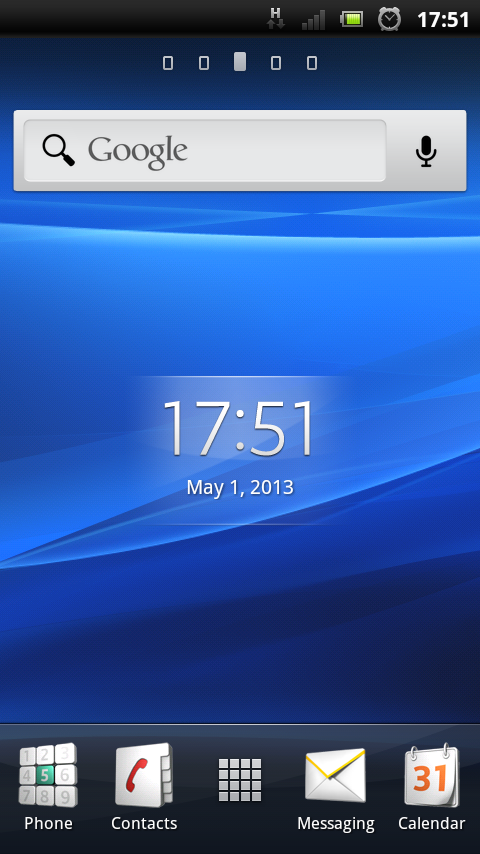
\includegraphics[scale=0.20]{part_2/context_awareness/screenshot_2013-05-01_1751.png}
    	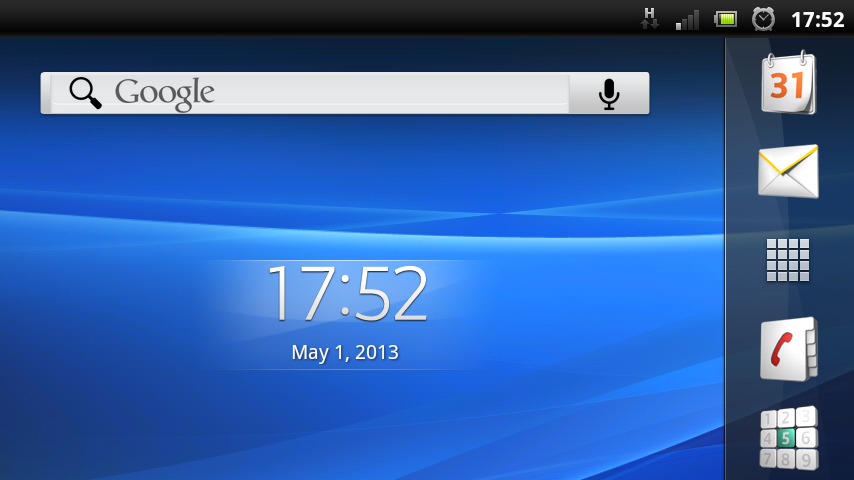
\includegraphics[scale=0.20]{part_2/context_awareness/screenshot_2013-05-01_1752.png}
		\caption{Android homescreen on a Sony Ericsson Xperia PLAY rotates based on context information from its sensors when the phone is 	physically rotated.} 
		\label{androidorientation}
\end{figure}

\section{Pervasive \& Ubiquitous Computing}
Pervasive and Ubiquitous computing describes the philosophy of "everything everywhere computing". To build context-aware applications context information is needed and ubiquitous computing can be used to make collection of this data possible.
Computers today are everywhere; in phones, TVs, cars, kitchen machines, watches, etc. Jens Malmodin et al. \cite{fehske2011global} predicts that 50 billion devices will be connected together by 2020. When computers become pervasive and ubiquitous it becomes important to make the computers themselves smart and easy to use instead. According to Mark Weiser in \cite{237456} the goal of Ubiquitous is 

\begin{quotation}
\centering
[...] the enhancing computer use by making many computers available throughout the physical environment, but making them effectively invisible to the user.
\end{quotation}

According to The Swedish Data Inspection Board \cite{datainspect}, ubiquitous computing is a new computer era. In the past one human only had one computer, so called personal computer (PC). In the last years this have been changing. Computers have been integrated into artefacts that humans use in their everyday life. Shoes can contain a computer chip that collects data about your running \cite{saponas2006devices}. With ubiquitous computing places and physical objects will be connected and communicate with each other and humans. 

If computers will be everywhere, they must be as small as possible. They also need to be cheap and be low-powered computers \cite{datainspect}. An example is the Raspberry Pi, a credit card sized computer that can be run with 4 x AA batteries. According to Moore's Law, in the coming years devices will be smaller, more powerful and they will be much cheaper \cite{591665}. This gives a good chance that computers which already are embedded in all things around us will be powerful enough to run multiple context aware applications.

%\section{Tendency Towards Resource Constrained Devices}
Alan Messer et al \cite{alanmesser} have identified a problem with the concept of pervasive computing. Peoples vision is to execute a service on any device without worrying about whether the service is designed for the device. Alan Messer et al suggests that it will be difficult to create a service that can be run on all devices due to the resource constraints on different devices. Devices differ from each other with respect to their processing power, available memory or network access, hence services need to be tailored to work on different devices.


A lot of existing computer software was first developed for computers with high resources. When software runs on a computer with low resources it needs a redesign to fit on the device. The operating system Android is built on Linux which was an operating system that first was used on personal computers. Android Inc redesigned the operating system to fit it on smartphones. The same goes for Microsoft that has developed a version of Windows for tablets and smartphones. Applications like Netflix, Google Chrome and Utorrent have been redesigned to fit different devices. Software can sometimes be run on a device for which it wasn't designed to run on, but the software is not tailored for those devices and will therefore be less efficient causing reduced performance.


%\section{Tendency Towards Resource Constrained Devices}
Alan Messer et al \cite{alanmesser} have identified a problem with the concept of pervasive computing. Peoples vision is to execute a service on any device without worrying about whether the service is designed for the device. Alan Messer et al suggests that it will be difficult to create a service that can be run on all devices due to the resource constraints on different devices. Devices processing, memory, network, power capacities differs from each other and services need to be tailored to fit on different devices. 

A lot of existing computer software was first developed for computers with high resources. When software runs on a computer with low resources it needs a redesign to fit on the device. The operating system Android is built on Linux which was an operating system that first was used on personal computers. Android Inc redesigned the operating system to fit it on smartphones. The same goes for Microsoft that has developed a version of Windows for tablets and smartphones. Applications like Netflix, Google Chrome and Utorrent have been redesigned to fit different devices. Software can sometimes be run on a device for which it wasn't designed to run on, but the software is not tailored for those devices and will therefore be less efficient causing reduced performance.

\section{Applications Using Context Information}
To build this big network of context aware applications that interact with users without them knowing it, some conditions must be understood. Because of the mobility of the devices the context information need to be collected and shared through wireless network. Moreover, the infrastructure for an Internet of Things platform have to scale well to increase amounts of users and have to always be available to these users \cite{Kanter539187}.

Another condition to consider is the large number of applications that should be able to run on a single ubiquitous device. The ubiquitous devices have limited performance, even if the evolution of the hardware is going forward. Due to their size it is important for an application to be lightweight. Ubiquitous computer devices have limited processing capability, small memory space and have limited battery time. The capability of processing is limited which make them not well suited for computation of intensive tasks. A ubiquitous device also has limited amount of available memory. This two conditions makes it more important to have lightweight applications and services on ubiquitous devices. As mentioned before battery time is also limited, for example the battery time is decreased whenever the device has network communication. Therefore it is important to make the applications and services efficient in the use of network communication. 
If we run a context-aware application on a Raspberry Pi we need to consider that the device only has 512 MB RAM and that this device should be able to run several instances of similar applications so the footprint from the network communication need to be reduced. 

The applications also need near instant access to context-information. Context-information need to be accessed in real-time to provide updated data from sensors. This cannot be provided with a centralized solution \cite{TheMediaSenseFramework}. Real-time delivery of context-information between endpoints is important to existing and future mobile applications. 

\section{Sharing the Information}
As the network of ubiquitous computers grows bigger, the amount of context information will increase as well, and it becomes necessary to understand how this information can be shared. When billions of users and applications is connected to the infrastructure, it is important to get the most effective and scalable solution for storing and sharing this kind of data. Applications will need to be able to access data in real-time, so the users get the most updated context information. 

To share the information ubiquitous devices need a middleware, a platform that can run on the ubiquitous devices and enable information sharing. This middleware should be able to provide the functionality for collecting and sharing context information, it also needs to be able to share the context information in real-time. Because of the ubiquitous devices resource limitations it needs to be lightweight and use the resources in an efficient way. There are two approaches this middleware could use to share context information, centralized and distributed.

\subsection{Centralized}
With centralized middleware solutions, the data is hosted and managed on a server, and if a device needs to store or access context information it has to connect to this server. One advantage of the centralized approach is that a server can be updated, with new hardware and software, to improve its performance. 
However, a server can only handle a certain amount of requests per second. To handle the larger quantities of requests, more servers will be required causing the costs to increase with the amount of users. A centralized approach is vulnerable to failures like attacks and crashes. When the server goes down, users won't be able to retrieve context information. Some examples of Internet of Things middleware which use this approach are SenseWeb \cite{senseweb} and Xively \cite{xively}.

%\begin{figure}[t]
%	\centering
%    	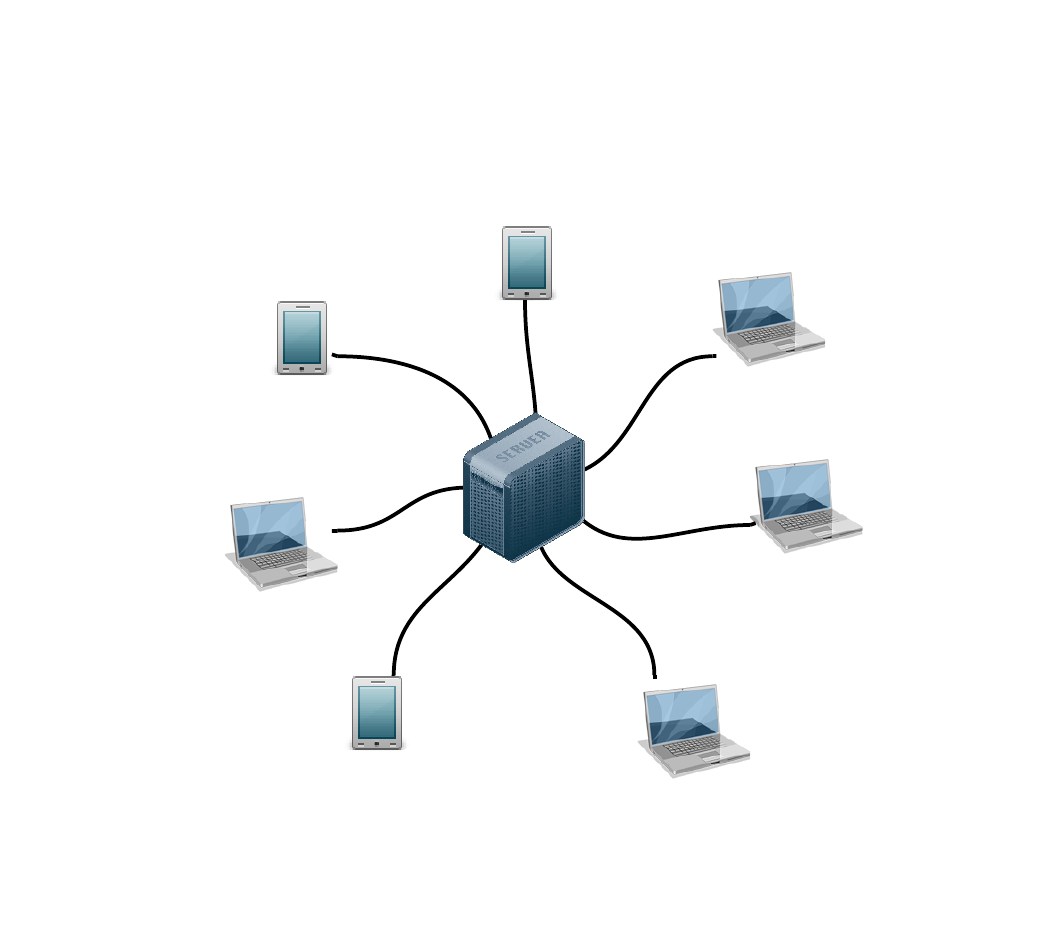
\includegraphics[scale=0.25]{part_2/sharing_the_information/Centralized.png}
%		\caption{Overview of a centralized network} 
%\end{figure}

\subsection{Distributed}
Distributed solutions allow computers / nodes to communicate with each other and share information and resources without using server computers. This is commonly used in file sharing software applications, such as Gnutella. Distributed solutions are more reliable and lack a single point of failure. Distributed solutions scale well compared to centralized solutions. Ubiware \cite{osterle2010memorandum} and MediaSense \cite{TheMediaSenseFramework} are both distributed Internet of Things middleware. 

%\begin{figure}[t]
%	\centering
%    	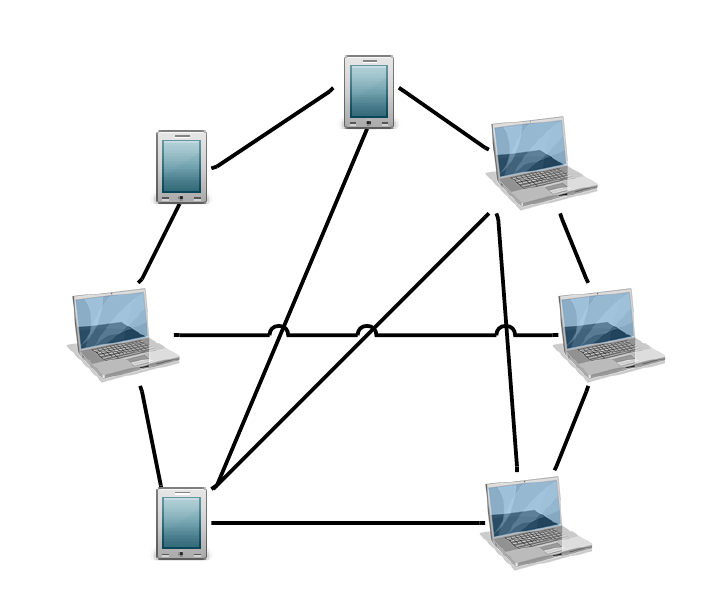
\includegraphics[scale=0.25]{part_2/sharing_the_information/Decentralized.png}
%		\caption{Overview of a decentralized network} 
%\end{figure}

\section{MediaSense}
MediaSense is a distributed middleware platform for the Internet of Things. It provides a scalable platform with a real time access to context information \cite{Kanter539187}. MediaSense allows support for applications and services to collect and share context information. This in turn enables users to focus on developing applications and services without needing to focus on how the context information is shared and how the layers in the platform is interacting with each other \cite{Walters413794}. 

\subsection{Distributed}
MediaSense is using a distributed peer-to-peer overlay to connect all the endpoints in the network. Context information is then persisted and shared in real-time among the nodes in the network. Each node in the network is both a producer and consumer enabling bidirectional access to context information. The overlay used is P-Grid \cite{aberer2003p}. With a lot of users running applications and sharing context information it is critical that the overlay structure is reliable and scalable \cite{aberer2003p}. P-Grid is self organizing allowing it to scale well. 

\subsection{Applications}
MediaSense is written in the programming language Java and provides an API that can be used to communicate with the platform. The communication from one platform on a device to another device running the platform is done with messages. The API provides methods for registering new context information and find nodes holding specific context information. Each node attached to the network generates information on a continual basis that is accessed and used by other nodes wishing to do so. In order to do this each node register UCIs (Universal Context Identifier). The UCI is stored in the distributed network and other nodes can resolve this and get the address where some required information is stored. When a MediaSense instance gets a message the dissemination layer in MediaSense handles this message and sending it to the application. The dissemination layer acts like a router delivering messages to the right place. Applications have a method for handling messages that is routed from the dissemination layer. 

\begin{figure}[t]
	\centering
	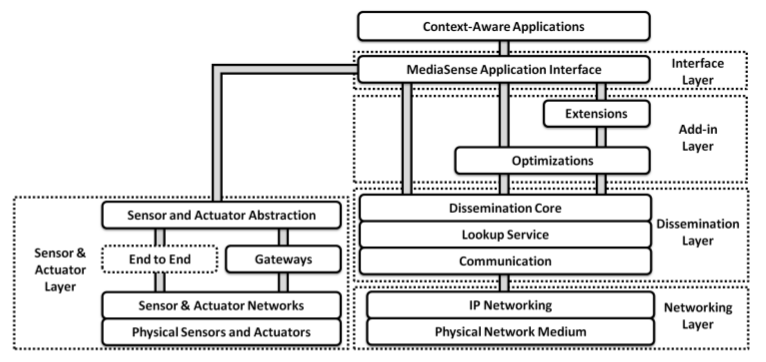
\includegraphics[scale=0.50]{part_2/mediasense/ms_arch.png} 	
	\caption{MediaSense component architecture \cite{Kanter539187} }
\end{figure}

\subsection{Messages}
As mentioned MediaSense communicates with messages. Applications can register what messages they are interested in. When the platform gets a new message from another node in the network the message will be handled by the dissemination core which then sends the message to the application on the platform interested in this message. There are several types of messages. The table \ref{tab:table} shows the primitive messages that are available for registering and retrieving information. 

\begin{center}
\begin{table}
    \begin{tabularx}{\textwidth}{ | l | X |}
    \hline
    Message name 		& 		Description \\ \hline
	REGISTER UCI 		& 		Registers a UCI along with the node which is responsible for it. \\ \hline
	RESOLVE UCI 		& 		Resolves a UCI to the node which is responsible for it. \\ \hline
	GET 				& 		Fetches the current context value from the node responsible for a UCI. The reply is sent using a NOTIFY. \\ \hline
	SET 				& 		Changes the current status of an actuator in an end point. \\ \hline
	SUBSCRIBE 			& 		Makes a subscription request to the node responsible for a UCI, The node then sends a NOTIFY message containing the current context value, either at regular intervals or when the value changes. \\ \hline
	NOTIFY 				& 		Notifies an interested node of the current context value associated with a specified UCI. \\ \hline
	TRANSFER 			& 		Requests the manager of a resource to transfer responsibility to another node. This might be full responsibility or partial, where the requester re-creates a copy of the resource permitting improved real time performance. \\ \hline
    \end{tabularx}
	\caption{Primitive messages in MediaSense}
	\label{tab:table}
\end{table}
\end{center}


\subsection{MediaSense Execution}
When an application wishes to use the MediaSense platform, the application must initialize and use its own instance of MediaSense. Therefore a user running two application at the same time must initialize two instances of the platform. Every instance of MediaSense is seen as a separate node, so if we have two instances of the platform on one device this device is acting as two nodes in the network. This is misleading because one node in the network should be one device and not one application.

\begin{figure}[t]
	\centering
    	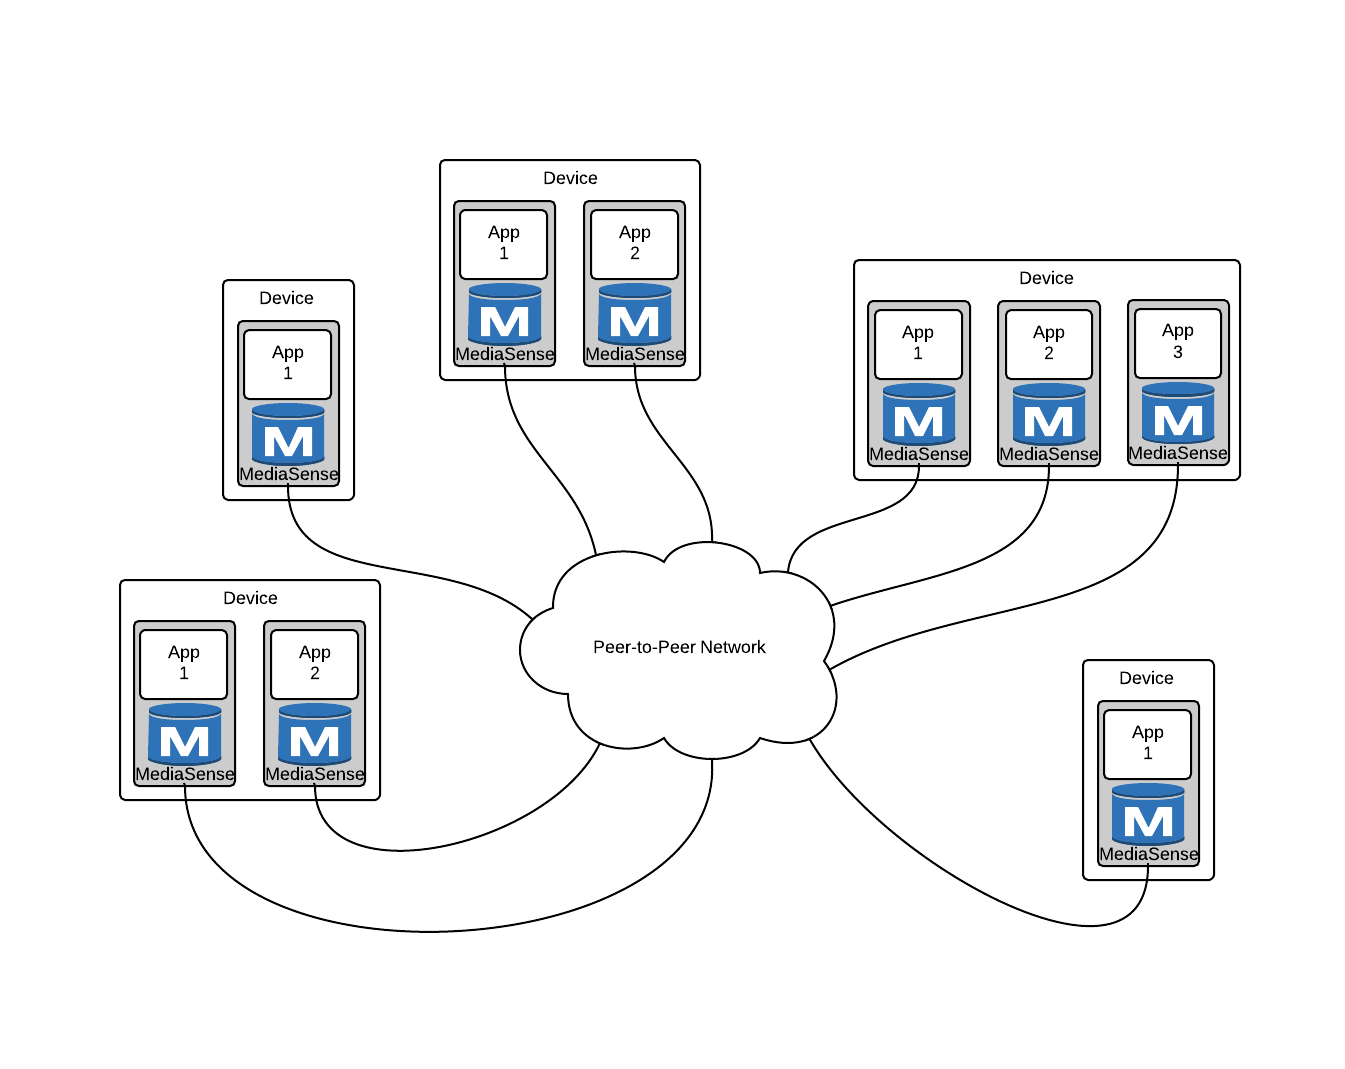
\includegraphics[scale=0.25]{part_2/mediasense/several_nodes_on_one_device.png}
		\caption{Figure showing how the instances of MediaSense is connected to the network} 
\end{figure}

Each instance of MediaSense requires that a new port be opened so the network layer can communicate with other nodes in the network. This means that if the user is behind a NAT or a firewall the user needs to open up new ports for every instance of MediaSense. The amount of open ports is equal to the amount of applications running on a device. This is a security issue. With more ports opened the device that is running the platform is more vulnerable. Not only that the device will be more vulnerable, when a user need several instances of MediaSense and every instance need its own port the network usage will increase. This can affect the battery time of low resource devices in a negative way.

One more thing to consider with an application invoked platform is that the memory usage will increase. Every instance of MediaSense need to use a specific amount of memory. If the platform is running on a resource constrained device this will limit the number of applications running on the device, because of the several instances of MediaSense. This is contradictory to the requirement defined by Kanter et al. \cite{Kanter539187} that Internet of Things Middleware should be lightweight.

To make MediaSense more efficient we need to reduce the resource footprint, without losing  the functionality. This can be done in several ways. One way is to change the overlay architecture and use a centralized approach for sharing and collecting context information. This solution will make every application connecting to a centralized server or to use a internet portal, for example RESTful API to access the data. The problem with this is that they are centralized and therefore not well scalable and we will lose the functionality of P-Grid. They are also dependent on DNS which means that applications expect that the centralized server are always available. As mentioned before centralized solutions are more vulnerable and can be attacked with Denial-of-service attacks. If the centralized server is having DNS errors the context information can not be accessed and shared to other applications and the applications is usable. Examples of Internet of thing services using this architecture is SenseWeb and Sensei. This two examples is using centralized web-services for sharing context information which makes them having the mentioned issues and are therefore not a good solution for an Internet of things service.

\begin{center}
\begin{table}
    \begin{tabularx}{\textwidth}{ |X|X|X|X| }
    \hline
    Number Of Applications 								& Memory Usage 									& CPU Time							& Threads\\ \hline
    1 													& 70.4 MB 										& 2.70 								& 30 \\ \hline
    2 													& 139.2 MB										& 5.34 								& 60 \\ \hline
    3 													& 213.04 MB										& 8.72 								& 90 \\ \hline
    4 													& 286.5 MB										& 12.88 							& 120 \\ \hline
    5													& 360.2 MB										& 15.43  							& 150 \\ \hline
    6													& 430.3 MB										& 18.82  							& 180 \\ \hline	
    7													& 505.3 MB										& 21.54  							& 210 \\ \hline
    8													& 574.1 MB										& 24.85  							& 240 \\ \hline
    9													& 648.3 MB										& 27.84	  							& 270 \\ \hline
    10													& 718.3 MB										& 31.25  							& 300 \\ \hline
    \end{tabularx}
   	\caption{This table shows how much resource is in use when MediaSense is running}
	\label{tab:test_table}
\end{table}
\end{center}
\section{Shared Resources to Reduce Resource Costs}
The resources of computers can be used in an effective way if the applications have resource consuming components located in a shared service. A shared service can act like a container where components like databases, calculations and network communication can be shared between all processes. One example of shared resources are web browsers. In the late 1990s and early 2000s web browsers could only visit one web page and to view multiple web pages simultaneously new windows had to be opened. Tabbed browsing or TDI (tabbed document interface) of web pages was popularized by Mozilla FireFox in 2003 and made it possible to have several web pages opened in one window. Tabbed browsing allows web browsers share services between the tabs displaying web pages. Examples of such services in web browsers are JavaScript engines, rendering engines, plug-ins, extensions, et cetera. 
MySQL has a shared service for all databases running on a server, a so called daemon, which handles access to all databases on the server. For example, the communication with MySQL is handled by the shared service which listens to a TCP port. When the service gets a request to this port it forwards it to the addressed database. If MySQL instead had one service for every database, one network layer is needed for every database which increase the resource usage. 

The tendency to gather resource consuming processed in one place and share access to them between many processes is the basis of the client-server model. Examples of such behaviours are numerous and prominent within the world wide web. Google's massive indexed database of web pages can be queried by millions of users at a time. This forces google to have large and powerful data centers to accommodate the users instead of each user downloading a copy of Google's database and querying it locally. Spotify's large collection of music can be accessed by users and streamed to a client giving access to approximately 80 terabytes (20 million songs at an average size of 4MB) of music for which the storage costs alone would be unfeasible for the average user by todays standards.
\section{Inter-Process Communication}
Inter-process Communication (IPC) is a term describing communication between two processes through a shared interface. There are a number of variations of IPC. In operating systems like Unix and Windows there are a mechanisms for local IPC such as files, sockets, pipes, shared memory and semaphores. 
Inter-process communication using files is simply done by two processes reading and writing to one or more files. Pipes are a way of directing the output of one program to the input of another program. A variation of pipes are named pipes, also called FIFO (first in first out) which are system persistent pipes, often represented as files \cite{Lewandowski97interprocesscommunication}. Sockets are software abstractions to create a bidirectional channel between processes. They come in two variations, datagram sockets and stream sockets. Datagram sockets are faster than stream sockets but less reliable \cite{Lewandowski97interprocesscommunication}. Shared memory allows two processes to access the same memory and semaphores are used to signal availability of a resource between processes to avoid information loss, so called race conditions, while writing to the same block of memory from two different processes.

For communication between applications there are Inter-process communication implementations supporting communication with applications running on remote computers through interfaces of a higher abstraction than those for local IPC. These can also be used locally but the abstractions come at a cost in resources.

Remote IPC can be done in two ways unicast and multicast. Unicast is when the communication is sent from one entity and received by another entity. An example of unicast remote IPC is Remote Procedure Calls, RPC. Multicast is when the communication is sent from one entity and received by a group of entities. An example of multicast IPC is message passing which is used by the MediaSense platform to communicate between nodes over the Internet.

\subsection{Message Passing}
Message passing performs IPC by sending and receiving messages. Received messages are placed in a queue and are handled asynchronously.
The messages contain data which is used to determine the action or response. This allows the receiver to prioritize some messages. Message passing provides few abstractions for the developer and requires the data to be marshalled before sending messages and unmarshalled before receiving messages. 

The Message Passing Interface, MPI \cite{mpi3stand}, is one such standardized message passing implementation. Sending and receiving operations in MPI can be either blocking or non-blocking. Blocking send and receive operations wait for the application buffer to be free for reuse before returning to prevent race conditions, while non-blocking messages allow the process to proceed as soon as possible.

\subsection{Remote Procedure Calls}
Remote Procedure Calls (RPC) are a form of IPC that allow one process to invoke a callable unit \cite{Eac} located in another logical or physical space. Usage of RPC makes it possible to both interact with programs running on the same physical memory and with applications located within the same network. RPC is an abstraction built on top of message passing to enable calls to remote procedures as if they were made locally.
RPCs are unicast and synchronous, the sender waits for a response from the recipient before continuing the execution. Remote procedure calls are handled as if the calls were done locally, the calling process waits for a return value before proceeding, see Fig. \ref{rpc}.

Bruce Jay Nelson first defined Remote Procedure Calls as
\begin{quotation}
\centering
[...] the synchronous language-level transfer of control between programs in disjoint address spaces whose primary communication medium is a narrow channel.  \cite{Nelson:1981:RPC:910306}
\end{quotation}

\begin{figure}[t]
		\centering	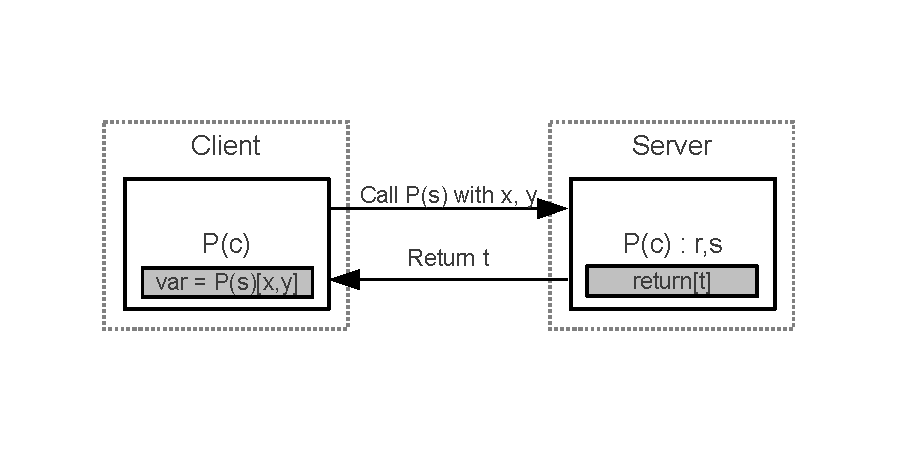
\includegraphics{part_2/remote_procedure_calls/rpc.pdf}
		\caption{Abstract of the events involved in remote procedure calls from a user perspective.
The procedure P(c) in the Client calls procedure P(s) located at the Server. The procedure P(s) receive two arguments r and s and return the value t which is stored in variable var back in the client.}
		\label{rpc} 
\end{figure}

When using remote procedure calls, one process is considered the server and one the client. The client is the caller process and the server receive and handle the process and then returns the value. The client and server both have stubs, server-side stubs are called skeletons. Stubs are modules in charge of marshalling the calls, which means packing the parameters of the call in a way that allows them to be stored or transferred via TCP or UDP \cite{rfc5531}. 
The events that occur when a client invokes a remote procedure call start with a call to the client's stub are shown in \ref{rpcflow}. The client stub receive the parameters from the local call and then marshalls. The marshalled data is then sent to the server by the the client's operating system. The server operating system receives the message and sends it to the skeleton. The skeleton unmarshalls the message  to obtain the parameters and invokes the local version of the procedure with the parameters. The server's procedure returns a value which is then sent to the skeleton. The skeleton then in turn marshalls the return value and sends the marshalled data back to the client. The client receives the message, the client stub unmarshalls the return value which then is sent back to the client's procedure \cite{Lewandowski97interprocesscommunication}. RPC implementations often is language specific. Some implementations, like XML-RPC and 
JSON-RPC use a common format for describing objects and can therefore be used cross-platform.

\begin{figure}[H]
		\centering	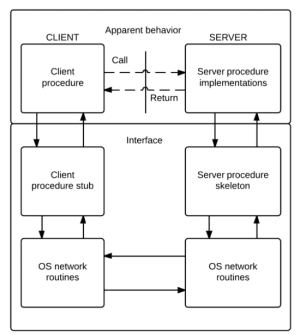
\includegraphics{part_2/remote_procedure_calls/Rpcflow300.png}
		\caption{The flow of a RPC}
		\label{rpcflow} 
\end{figure}

\subsection{Remote Method Invocation}
Remote method invocation (RMI) is a Java implementation of RPC with support for Java objects and allows entire objects to be passed and returned as parameters instead of only primitive data types. These objects can be dynamically loaded in the receiving Java Virtual Machine and can therefore be of an object type unknown to the receiver. RMI requires objects to be RemoteObjects, a remote object must implement a remote interface to support remote invocations. When a remote object is sent to another Java Virtual Machine it is sent as a remote stub to the receiving remote.
RMI relies on a registry to find other remote objects which have to be registered with a name. Other objects can then do a lookup on the registered name to get a reference to the Remote object. RMI registries can be shared between multiple JVMs on the same machine which facilitates communication from newly created processes to persistent ones.

\begin{figure}[H]
	\centering
    	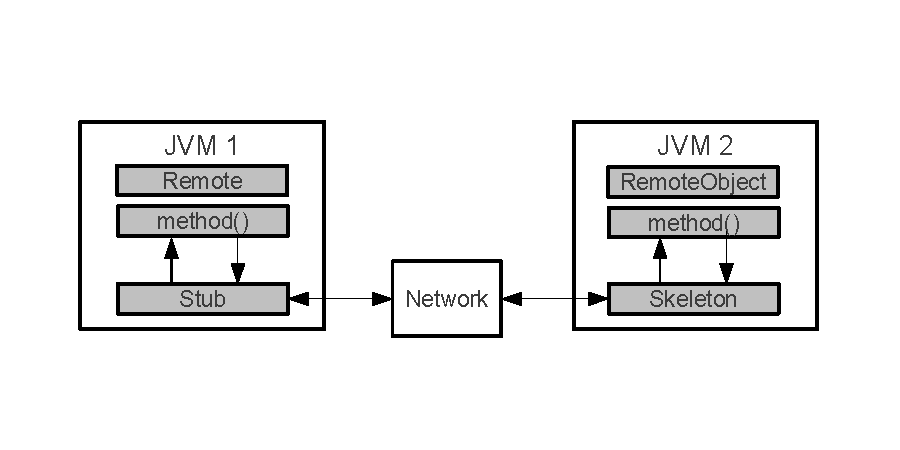
\includegraphics{part_2/remote_procedure_calls/rmi.pdf}
		\caption{The sequence of events in a method invocation with RMI.}
		\label{rmi} 
\end{figure}

\subsection{CORBA}
Common Object Request Broker Architecture is an object-oriented Remote Procedure Call mechanism. Corba is implemented in many different programming languages. This enables softwares written in different languages to communicate with each other. This is done with a language neutral API. CORBA uses an Object Request Broker which provides the mechanism required for distributed objects to communicate with each other. The Object Request Broker determines the location of target object, sends a request to that object and then returns a response back to the calling object. This communication is done over TCP/IP. However, in CORBA it is not possible to bind an Object Request Broker to a specific port. If the client is behind a firewall there is no option to change the port and use another port. This makes Corba firewall unfriendly.

